%----------------------------------------
% Preamble to set up the document
%----------------------------------------
\documentclass{article}

% set up packages (you shouldn't need to touch this)
\usepackage{listings}

\usepackage{graphicx}  % required to insert images
\usepackage{hyperref}  % for hyperlinks

\usepackage[svgnames]{xcolor}  % to change hyperlink colors
\colorlet{linkcolour}{DarkBlue}
\hypersetup{colorlinks=true, linkcolor=linkcolour, citecolor=linkcolour, urlcolor=linkcolour,}

% Margins
\topmargin=-0.45in
\evensidemargin=0in
\oddsidemargin=0in
\textwidth=6.5in
\textheight=9.0in
\headsep=0.25in
\usepackage{color}

%New colors defined below
\definecolor{codegreen}{rgb}{0,0.6,0}
\definecolor{codegray}{rgb}{0.5,0.5,0.5}
\definecolor{codepurple}{rgb}{0.58,0,0.82}
\definecolor{backcolour}{rgb}{0.95,0.95,0.92}
\lstdefinestyle{mystyle}{
  backgroundcolor=\color{backcolour},   commentstyle=\color{codegreen},
  keywordstyle=\color{magenta},
  numberstyle=\tiny\color{codegray},
  stringstyle=\color{codepurple},
  basicstyle=\footnotesize,
  breakatwhitespace=false,         
  breaklines=true,                 
  captionpos=b,                    
  keepspaces=true,                 
  numbers=left,                    
  numbersep=5pt,                  
  showspaces=false,                
  showstringspaces=false,
  showtabs=false,                  
  tabsize=2
}
\lstset{style=mystyle}

% use a sans serif font
\renewcommand{\familydefault}{\sfdefault}

%----------------------------------------
% Step 1: Edit the lecture title
%----------------------------------------
\title{
Lecture 8: Model complexity and generalization \\  % Lecture title
Modeling Social Data, Spring 2019 \\   % Course title
Columbia University                    % School
}

%----------------------------------------
% Step 2: Edit your name and the date
%----------------------------------------
\author{Chaim Eisenbach}                     % Scribe's name
\date{March 15, 2019}                % Lecture date

\begin{document}

\maketitle


%----------------------------------------
% Step 3:
% Rename uni.tex to match your uni,
% edit the filename accordingly below,
% and put your notes in this file
%----------------------------------------
%----------------------------------------
% Write your notes here
%----------------------------------------

\section{Introduction}
Deciding how complex your model should be and how to evaluate it. Phrase a linear model as an optimization problem.
Today we are discussing the ‘Art of Modeling’ 
the claim is that for most social science problems you don’t need fancy methods. When the features are really clear (age, income, etc.) linear models are usually good enough.
If you understand everything you can do with a linear model then more complex models are just a step away.
\section{notes}
 

 \href{https://github.com/jhofman/msd2019/blob/master/lectures/lecture_7/linear_models.ipynb}{Check Lecture 7 notebook} 
 
A few things to keep in mind when exploring this data set: Looking at a histogram of page views on a log-scale there is no place to put a zero. The really really high page view counts are probably bots or something. If we did not have a log-scale we would have a very low resolution.
Another key aspect of modeling is the readability of your plots in order to visualize the data you are manipulating.
So splitting the data into different groups can help. 

The users: (age, gender, daily views, median daily views) = 225,000 rows. 
The shaded area around the line, when using geom$\_$smooth, is capturing the uncertainty.
Now, instead of having ggplot2 do the modeling for us, let's do it ourselves.
\begin{lstlisting}[language=R]
model <- lm(log10(daily.views) - age, datamodel = data)
summary(model)
\end{lstlisting}
%(daily views) = $w_0$+ $w _1$. %where $w_0$ is the intercept and %$w_1$ is the slope.

The standard error is if you got different samples of the data how much would the coefficient vary.
$X \rightarrow \bar{X}_n ~~~ \sigma \rightarrow \sigma_{se} = \frac{\sigma}{\sqrt{n}}$

Bootstrap.
\begin{enumerate}
  \item Sample from data you have
  \item Estimate coefficient
  \item look at standard deviation of distribution of estimates
\end{enumerate}
So you do this a whole bunch of times and you'll build up some distribution  where $\hat{w}$ is our estimate and we look at the width of the distribution so the standard deviation of this distribution is the standard error on the coefficient estimate. If you have a small sample the distribution will be wider than if you had a large sample of data.
If you have enough data you'll get a really tight distribution and still a small standard error. 

There are a bunch of tidyverse functions

\begin{lstlisting}[language=R]
tidy(model)
glance(model)


tidy(model) %>%
    ggplot(aes(x = term, ye =estimate) +
    geum_pointrange(aes(ymin = estimate - stderror ...)) +
    facet_wrap(~ term, scale = "free_y")
\end{lstlisting}

$\hat{y} = w_0 + w_1x_1 + w_2 ...\\
\hat{y} = w_0 + w_1 \text{age} + w_2 \text{age}^2$
It's linear in the coefficients. But not necessarily the features themselves (the original features).
\begin{lstlisting}[language=R]
M <- model.matrix(log10(daily.views) ~ age + I(age^2), model_data)
## '+' means use this set of variables so 'I' forces a new feature which is age^2
head(M)
\end{lstlisting}
This is the actual set of numbers that go into our $X$ matrix. ($\hat{W} = (X^TX)^{-1} X^T y$). So we are just offloading all this onto a linear algebra library, because we are lazy and don't really have time for that. 
When we go into a non-linear world our ability to interpret the tables falls apart, but it's useful for plots.
Adding gender specific features means that the other gender is only explained by the unspecified features.
While the machine can do all these things it's up to you to figure out what to put in. There's a lot of creativity when constructing the model.

\vspace{0.3cm}

\href{https://github.com/jhofman/msd2019/blob/master/lectures/lecture_8/model_evaluation.ipynb}{Model evaluation} 

The more features the more crowded the plot and the harder it is to interpret or visualize.

\begin{lstlisting}[language=R]
ggplot(plot_data, aes(x = pred, y = geom_mean_daily_views, color = age)) +
  geom_point() +
  geom_abline(linetype = "dashed") +
  xlab('Predicted') +
  ylab('Actual') +
  facet_wrap(~ gender, scale = "free")
\end{lstlisting}
We don't have that many points because we are taking the averages.

But now we can see how terrible this model is
%\begin{lstlisting}[language=R]
%pred_actual <- model_data %>%
%  add_predictions(model) %>%
%  mutate(actual = %log10(daily.views))

%ggplot(pred_actual, aes(x = %10^pred, y = 10^actual)) +
%  geom_point(alpha = 0.1) +
%  geom_abline(linetype = %"dashed") +
%  scale_x_log10(label = comma, %breaks = seq(0,100,by=10)) +
%  scale_y_log10(label = comma) +
%  xlab('Predicted') +
%  ylab('Actual')
%\end{lstlisting}

%Figure %\ref{fig:figures/ScreenSho%t} is an example of how to %include an image.

\begin{figure}[ht]
  \begin{center}
    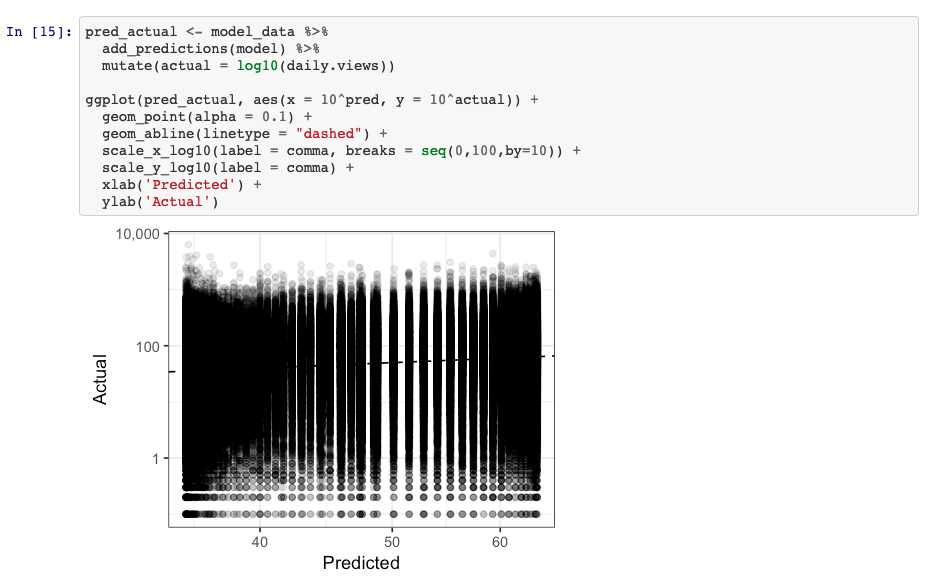
\includegraphics[width=1.0\textwidth]{figures/ScreenShot.png}
    \caption{
      The variance is crazy and this model is good for nothing.}
    \label{fig:example_figure}
  \end{center}
\end{figure}


We can also quantify how well this does. 
MSE-{model} $ = \frac{1}{n} \sum_{i-1}^n (y_i - \hat{y}_i)^2$, RMSE-model $= \sqrt{\text{MSE}_{\text{model}}}$, ($var(y)$) = MSE-baseline(mean) $= \frac{1}{n}\sum_{i=1}(y_i - \bar{y})^2$. $\frac{MSE-baseline - MSE-model}{MSE - baseline} = R^2$ which is the fraction of variance explained. 

In R:
\begin{lstlisting}[language=R]
rmse(model, model_data)
rsquare(model, model_data)
\end{lstlisting}

\href{https://github.com/jhofman/msd2019/blob/master/lectures/lecture_8/lecture_8.pdf}{Check Lecture 8}

Bias-Variance tradeoff. A linear model is biased because it can only find linear trends. But it does not vary a lot with different samples of the data. High bias, low variance.  As the model gets more complicated you can have a better fit. At some point there's a sweet spot with enough complexity and a good balance of bias-variance. 

\begin{figure}[ht]
  \begin{center}
    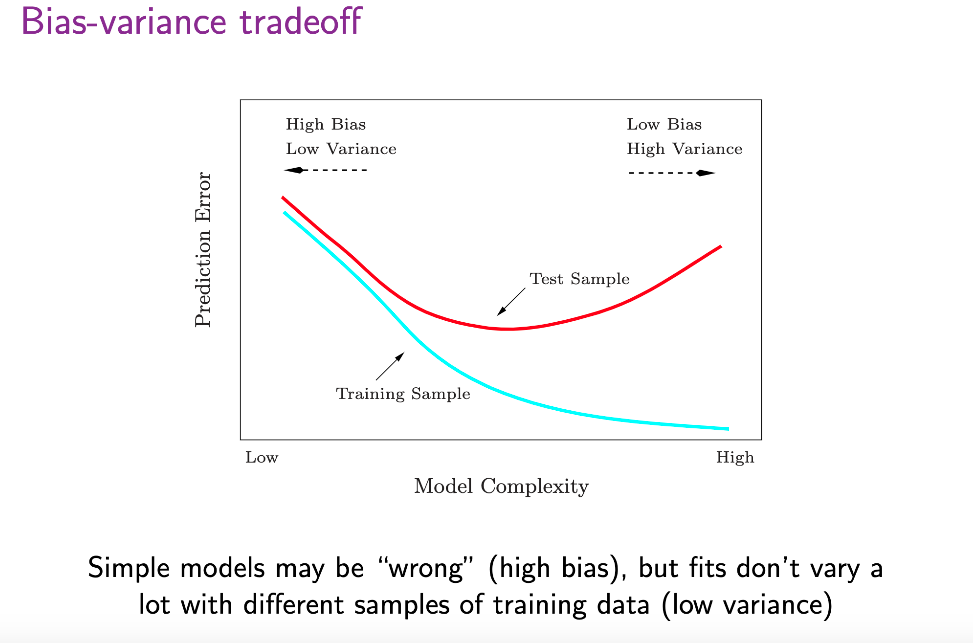
\includegraphics[width=1.0\textwidth]{figures/ScreenShot2.png}
 
  \end{center}
\end{figure}

Cross-validation. You can train it one one subset and test the model on another, never seen, subset of the data.

\href{https://github.com/jhofman/msd2019/blob/master/lectures/lecture_8/complexity_control.ipynb
}{Complexity control}


$\frac{1}{n}\sum_{i=1}^n (y_i - w x_i)^2 (which ~is~ the~ fit) + \lambda ||{w}||^2 (size~ of~ coefficients,~ tradeoff~ between ~ fit ~ and ~ complexity)$ 
So we have our hyperparameter $\lambda$ which is what we need to determine to find the best model. We can do this through various testing techniques. 
\href{https://github.com/jhofman/msd2019/blob/master/lectures/lecture_8/intro_to_glmnet.ipynb}{Into to glmnet} what glmnet does is figure out the paremeters in our fit to the data above
So even if you give it something crazy like a 10th degree polynomial it will return something normal.

"Weird R things with the dots, it's just terrible" - Jake Hofman


\end{document}

%%% Local Variables:
%%% mode: latex
%%% TeX-master: t
%%% End:
